\documentclass[a4paper, 11pt]{article}

%% Language and font encodings %%%%%%
\usepackage[utf8]{inputenc}
\usepackage[T1]{fontenc}
\usepackage[french]{babel}

%%%%%%% Page Size, Geometry and Margin Size %%%%%%%%%
\usepackage[a4paper,top=2cm,bottom=2cm,left=2cm,right=2cm,marginparwidth=2cm]{geometry}

%%%%%%% USEFUL PACKAGES %%%%%%%%%
\usepackage{enumitem}
\usepackage{minted} % Allow for code style
\usemintedstyle{vs}%{borland} 
\usepackage[dvipsnames, svgnames, table]{xcolor}    % Allow to use colors (even within tables)
\usepackage[colorlinks=true, linkcolor=blue, urlcolor=blue, hyperfigures=true]{hyperref} % Allow to make cross-references and links
\usepackage{graphicx} % Allow to insert figures
%\usepackage{subfigure}
\usepackage[format=hang]{caption} % Caption for figures
\usepackage{subcaption}
\captionsetup{format=hang, labelfont=bf}
\usepackage{amsmath}
\usepackage{amsfonts}
\usepackage{amssymb}


\begin{document}
%%%%%%%%%%%%%%%%%%%%%%%% TITLE PAGE %%%%%%%%%%%%%%%%%%%%%%%%
\begin{titlepage}
\newcommand{\HRule}{\rule{\linewidth}{0.5mm}} 							% horizontal line and its thickness
\center
~\\
\vspace{8cm}

\HRule \\[0.5cm]
{ \huge \bfseries  SYST0002 - Introduction aux signaux et systèmes\\ ~\\ \Large Rapport de projet}\\[0.5cm]								
\HRule ~\\[2cm]
\large
\vspace{5cm}


{\Large
\begin{flushleft}
\begin{tabular}{l|l}
    Professeurs & Guillaume Drion \& Alessio Franci\\
    Assistants & Antoine Debor \& Caroline Dejace \\
    Auteurs & {Justin Jacquemin} \& {Loic Delbarre}\\
    Matricules & S{224395} \& S\textcolor{red}{XXXXXX}
\end{tabular}
\end{flushleft}
}


\vfill
\begin{center}
    \textsc{Année académique 2024 - 2025}    
\end{center}

\end{titlepage}
%%%%%%%%%%%%%%%%%%%%%%%%%%%%%%%%%%%%%%%%%%%%%%%%%%%%%%%%%%%%
\newpage
\section*{Part 1: Modèle d'état, linéarisation et simulations}
\begin{enumerate}
    \item 
    Le système dynamique est-il linéaire ? \\
Non, le système est non linéaire. Avec la présence de sinus, de tangente et d'arctangente, notre position en fonction du temps n'est pas linéaire. Ces fonctions ne sont ni additives ni homogènes, ce qui prouve que notre système n'est pas linéaire.

    \item 
    
Notre système dynamique est décrit par :  
\[
\frac{d}{dt} 
\begin{pmatrix} 
y(t) \\ \theta(t) 
\end{pmatrix} 
=
\begin{pmatrix} 
v_0 \sin(\alpha(\delta(t)) + \theta(t)) \\ 
\frac{v_0 \sin \alpha(\delta(t))}{a} 
\end{pmatrix}
\]
\[
\text{avec} \quad \alpha(\delta(t)) = \arctan \left( \frac{a \tan(\delta(t))}{b} \right)
\]

Nous constatons que le comportement du système dépend de plusieurs paramètres distincts.  

\subsection*{Paramètres fixes}  
Les premières constantes à considérer sont \( a \) et \( b \). Elles sont liées aux caractéristiques physiques du véhicule et restent invariables. Elles ne constituent donc pas des entrées du système.  

\subsection*{Influence de la vitesse \( v_0 \)}  
La vitesse \( v_0 \) pourrait également influencer la sortie \( s(t) \). Toutefois, puisqu'elle est supposée être constante au cours du temps, elle ne peut donc être considérée comme une entrée du système.  

\subsection*{Entrée du système}  
La seule variable candidate en tant qu’entrée est \( \delta(t) \), correspondant à l’angle de braquage des roues avant. Cet angle, variant en fonction du temps, influence directement la sortie \( s(t) \), ce qui en fait l’unique entrée du système.    

\section*{Analyse des sorties et des variables d’état}  

\subsection*{Sortie du système}  
D’après l’énoncé, l’unique sortie est \( s(t) \), correspondant à la position du module au cours du temps, soit \( y(t) \).  

\subsection*{Variables d’état}  
Les variables d’état décrivent l’évolution interne du système. Ici, nous avons :  
\begin{itemize}
    \item la position \( y(t) \),  
    \item l’orientation du module \( \theta(t) \).  
\end{itemize}

Ainsi, notre système dynamique possède :  
\begin{itemize}
    \item Une entrée : \( \delta(t) \).  
    \item Une sortie : \( s(t) = y(t) \).  
    \item Deux variables d’état : \( y(t) \) et \( \theta(t) \).  
\end{itemize}

\section*{Interprétation physique des signaux}  
\begin{itemize}
    \item \( y(t) \) représente la position verticale du centre de masse du véhicule au cours du temps. L'énoncé ne fixe aucune contrainte sur \( y(t) \), nous pouvons donc supposer que son domaine de définition ainsi que son image appartiennent à \( \mathbb{R} \).  
    \item \( \theta(t) \) représente l'orientation du module, soit l'angle entre l'axe horizontal et la direction du véhicule. Comme pour \( y(t) \), aucune contrainte explicite n’est donnée, mais dans un contexte physique, il est plus raisonnable de restreindre son image à l’intervalle \( [0, 2\pi[\).  
    \item \( a \) et \( b \) sont des constantes caractérisant respectivement :  
    \begin{itemize}
        \item \( a \) : la distance entre l'axe arrière et le centre de masse du véhicule.  
        \item \( b \) : la distance entre l’axe des roues avant et celui des roues arrière.  
    \end{itemize}
    \item \( v_0 \) représente la vitesse du centre de masse du véhicule.  
    \item \( \delta(t) \) est l’angle de braquage du véhicule, défini comme l’angle entre l’axe de la roue avant gauche et la direction du véhicule, soit \( \theta(t) \). Son image appartient à l’intervalle \( \left[ -\frac{\pi}{2}, \frac{\pi}{2} \right] \).  
\end{itemize}

Pour tous les signaux mentionnés, nous supposons que \( t \in \mathbb{R} \).  

\subsection{simulation du système}
\subsubsection{cas d'un mouvement sans tourner}
\begin{figure}[!h]
    \centering
    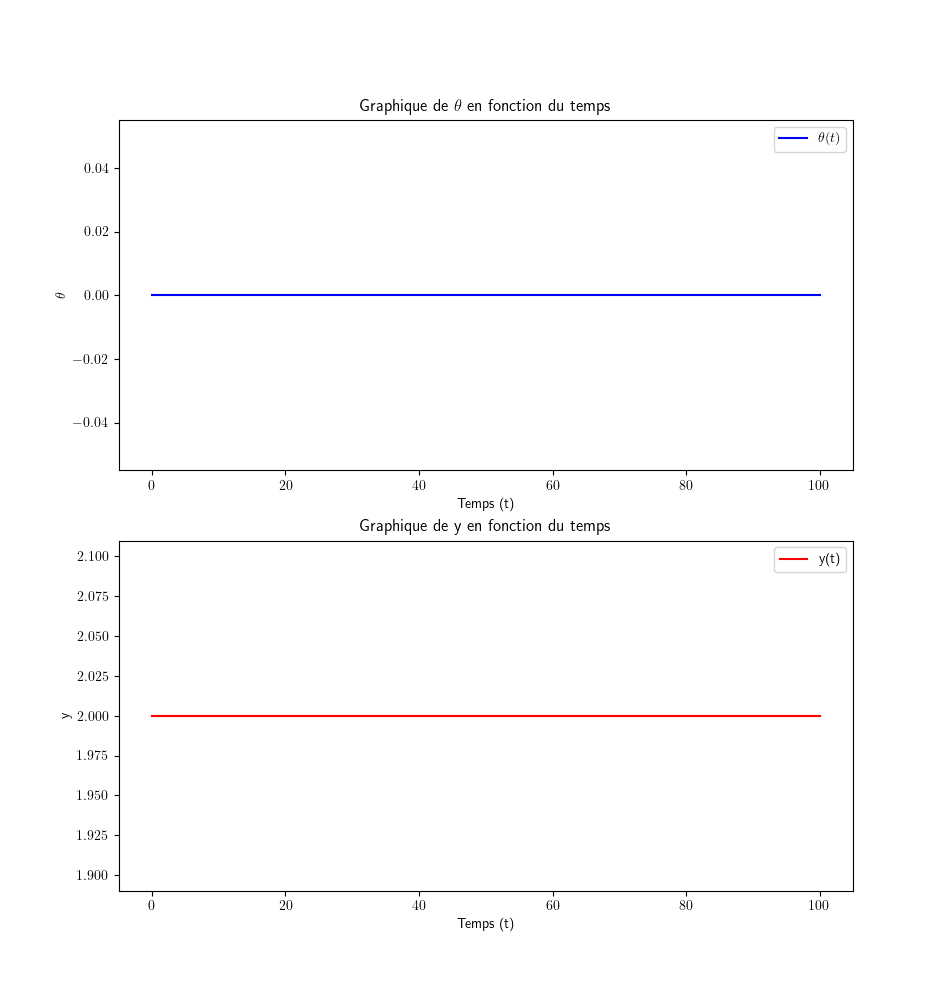
\includegraphics[width=0.5\linewidth]{Q3_flat.png}
\end{figure}
\newpage
\subsubsection{cas d'une mouvement dont les roues oscillent sinusoidalement}
\begin{figure}[!h]
    \centering
    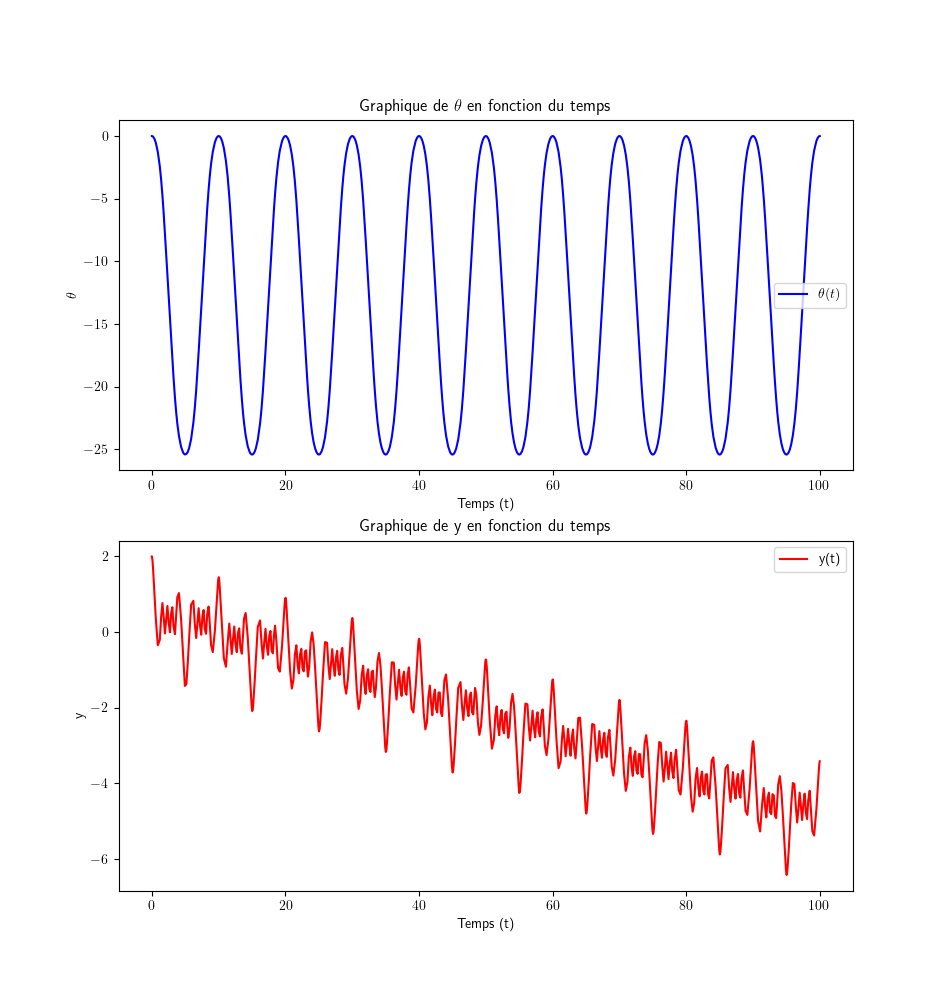
\includegraphics[width=0.5\linewidth]{Q3.png}
\end{figure}
    

    \item Pour trouver les points d'équilibre de notre système, nous devons résoudre un tel système : \[\dot{y} =v_0 \cdot  sin(\alpha(\delta(t) + \theta(t)) = 0\]
    \[\dot{\theta} =  \dfrac{v_0\cdot sin(\alpha(\delta(t))}{b} =  0  \]
    
    
    où \(\alpha(\delta(t))=arctan( \dfrac{a \cdot tan(\delta(t))}{b}\)
    et \(\delta(t)=\dfrac{-\pi}{2} \cdot sin(2\pi \cdot 0.1 \cdot t)\) ou = 0, comme decrit dans l'énoncé.\\
    Nous allons commencé par notre deuxième fonction qui nous permettra de trouver par la suite les points d'équilibre de la première fonction. 
    Nous devons donc partir de cette équations : 
    \[\dfrac{v_0 *sin(\alpha(\delta(t))}{a} = 0\]
    Nous savons que a \(\neq\) 0 nous obtenons alors simplement :
    
    \[sin(\alpha(\delta(t)) = 0\]
    
    \[\alpha(\delta(t) =k \pi \ , \  k\in \mathbb{Z}\]
    
    en remplacant \(\alpha(\delta(t))\) on obtient \[arctan(\dfrac{a\cdot tan(\delta(t)}{b})=k \pi \ , \ k\in \mathbb{Z} \]
    
    Cependant comme l'image d'un arctan est [\(\dfrac{-\pi}{2} \ ; \dfrac{\pi}{2}\)] la seule possibilite pour k est qu'il soit egal à 0. 
    On obtient donc facilement le point d'équilibre :
    \[ \dfrac{a \cdot tan(\delta(t))}{b} = 0\]
    
    \[\delta(t) = k'\pi \ , k' \in \mathbb{Z}\]
    En remplacement \(\delta(t)\) dans \(\dot{y}\) on trouve:
    \[v_0 \cdot sin( k\pi \ + \theta(t)) = 0\] 
    Et donc de manière similaire à la resolution précedente, on peut ecrire que \(\theta(t) = k\pi \ , k \in \mathbb{Z}\).\\
    Cependant les valeurs possibles de $\theta \in [0 \ , 2\pi[$ on a donc que les seul possibilités pour k est 0 et 1. De même que pour $\delta(t)$ les seuls possibilités a l'interieur de son interval de possibilité est k' = 0. Le systeme possede donc 2 points d'équilibre : $(\theta_{e1} \ , \delta_{e1}) \ = (0 \ , 0)$ ainsi que $(\theta_{e2} \ , \delta_{e2}) = (\pi \ , 0 ) $ Nous pouvons voir que les points d'équilibre ne font pas intervenir y(t) et donc nos points d'équilibre sont bon pour tout y(t).\\ 
    

    
    \item Afin de determiner les matrices A,B,C et D nous devons tout d'abord linéarisé notre systeme dynamique pour des petites perturbations. Nous supposons donc que \(\delta(t) \approx 0\), on peut donc alors approximer \(\alpha(\delta(t))\) en utilisant le développement de taileur.\\
    Approximation de \(\alpha(\delta(t))\)\\
    Comme décrit dans l'énoncé, \(\alpha(\delta(t))\) est donnée par 
    \[\alpha(\delta(t)) = arctan( \dfrac{a*tan(\delta(t) )}{b})\]
    Pour de petite valeurs de \(\delta(t)\), nous pouvons utiliser l'approximation tan(\(\delta(t)\)) \(\approx\) \(\delta(t)\), ce qui nous donne :   
    \[
    \alpha(\delta(t)) \approx \arctan\left(\frac{a\delta(t)}{b}\right)
    \]
    Ensuite en utilisant l'approximation de arctan(t) \(\approx t \) pour un petit t, on obtint : 
    \[
\alpha(\delta(t)) \approx \dfrac{a \cdot \delta(t)}{b}
\]
    Ensuite, en faisant toujours l'hypothese des perturbation, nous pouvons utiliser l'approximation de \(sin(t) \approx t\) pour x proche de 0 : 
    \[sin(\alpha(\delta(t)) + \theta(t) \approx \alpha(\delta(t)) + \theta(t) \approx \dfrac{a \cdot\delta(t)}{b} + \theta(t) \]
    et 
    \[sin(\alpha(\delta(t)) \approx \alpha(\delta(t)) \approx \dfrac{a\cdot\delta(t)}{b} \]

    On obtient alors notre system linéarisé et devient : 
    \[
\frac{d}{dt}
\begin{pmatrix}
    y(t) \\
    \theta(t)
\end{pmatrix}
=
\begin{pmatrix}
    v_0 \left(\frac{a}{b} \delta(t) + \theta(t) \right) \\
    \frac{v_0}{b} \delta(t)
\end{pmatrix}
\]
Ce qui peut s'écrire sous forme matricielle : 
\[
\frac{d}{dt}
\begin{pmatrix}
    y(t) \\
    \theta(t)
\end{pmatrix}
=
\begin{bmatrix}
    0 & v_0 \\
    0 & 0
\end{bmatrix}
\begin{pmatrix}
    y(t) \\
    \theta(t)
\end{pmatrix}
+
\begin{bmatrix}
    v_0 \frac{a}{b} \\
    \frac{v_0}{b}
\end{bmatrix}
\delta(t).
\]
Notre systeme étant plus lisible nous pouvons maintenant facilement determiner nos matrices : \\
Notre matrice A = 
\begin{bmatrix}
    0 & v_0 \\
    0 & 0 
\end{bmatrix}, B = 
\begin{bmatrix}
    v_0\frac{a}{b}\\
    \frac{v_0}{b}
\end{bmatrix}, C =
\begin{bmatrix}
    1 & 0 
\end{bmatrix}
et pour finir D = 0. Nous obtenons bien 4 matrices qui ont les bonne dimension.

    
  \subsection{nature des points d'équilibre}
La matrice Jacobienne pour les points d'équilibre est déterminé via
$ det(A-\lambda \mathbb{I})=0 $.On obtient donc que les valeur permisent pour lambda sont nulles.On ne peux donc rien conclure concernant la stabilité du système.
\subsection{simulation au point d'équilibre}



\begin{figure}[!h]
    \centering
    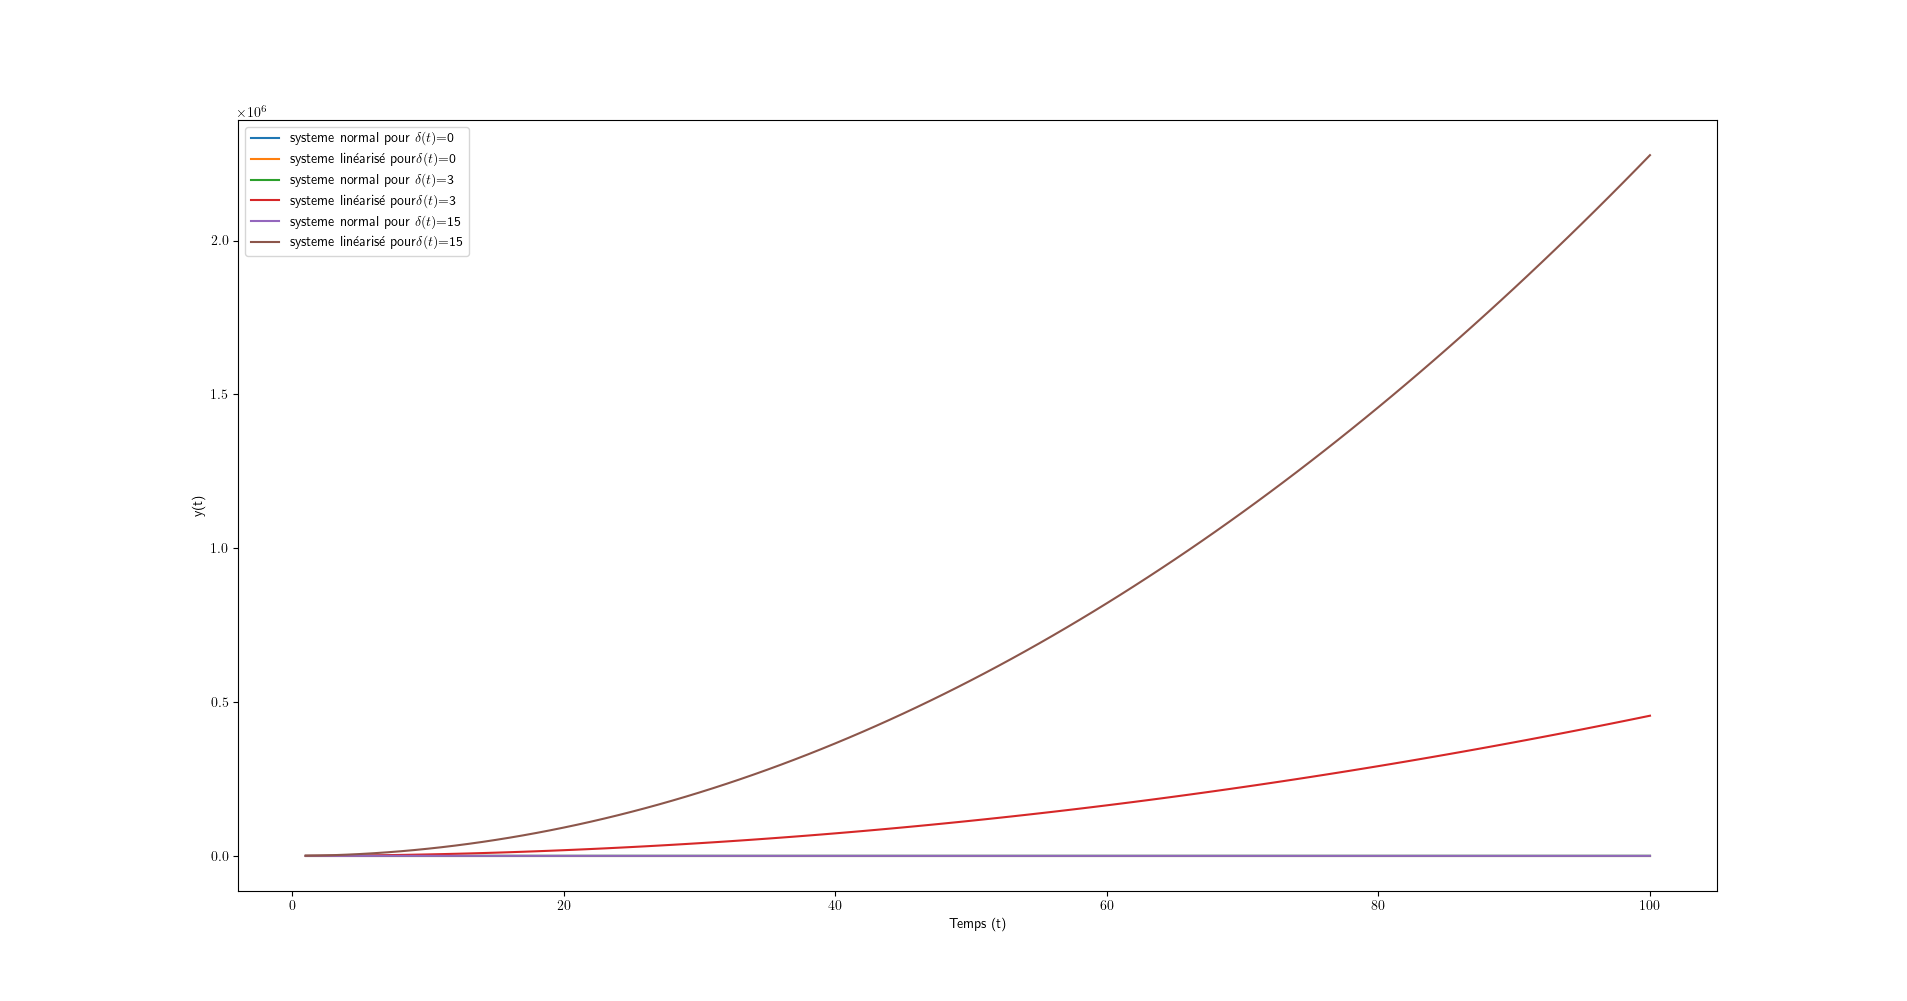
\includegraphics[width=0.5\linewidth]{Q7.png}
\end{figure}
On peut constater que les fonctions non linéaire ont le même résultat que celle du modèle ABCD.Vu que $\delta$ étant constant , la valeur de $\dot \theta$ n'est pas modifié au fur et a mesure du temps et donc pour $\theta>0 $ on appercois une augmentation de y(t) constante qui est représenté sur la courbe par la courbure exponentielle.










\subsection{trajectoire gaussienne}
Actuellement nous avons essayé plusieurs méthode sans parvernir à trouver une solution 
\subsubsection{résolution analytique}
On peut se pencher sur le système linéarisé , et deviner par identification quels facteurs permetteraient d'avoir le nombre et la valeurs des coefficient de nos gaussienne.
en réinjectant la deuxième équation linéarisé dans la première on se réduit à l'équation différentielle suivante:
$$\dot y = v_0 \dfrac ab  \delta + \dfrac{v_0} b \dot \delta $$
La solution recherché est 
$$y= \dfrac{25}{\sqrt{2 \pi \sigma^2}} exp(\dfrac{-(t-µ)^2}{2\sigma^2})$$
Sa dérivée par rapport au temps est donc
$$\frac{dy}{dt} = -\dfrac{25(t-\mu)}{\sqrt{2 \pi \sigma^2} \sigma^2} \exp\left(\dfrac{-(t-\mu)^2}{2\sigma^2}\right)$$
l'équation différentielle se réecrit donc :
$$-\dfrac{25(t-\mu)}{\sqrt{2 \pi \sigma^2} \sigma^2} \exp\left(\dfrac{-(t-\mu)^2}{2\sigma^2}\right) = v_0 \dfrac{a}{b} \sum^n_{i=0} \left( \dfrac{A_i}{\sqrt{2\pi\sigma_i^2}} \exp \left(\dfrac{-(t-\mu_i)^2}{2\sigma_i^2}\right) \right)+\dfrac{v_0}{b}\sum^n_{i=0} \left(-\dfrac{A_i(t-\mu_i)}{\sqrt{2 \pi \sigma_i^2} \sigma_i^2} \exp\left(\dfrac{-(t-\mu_i)^2}{2\sigma_i^2}\right)\right)$$
Si l'on considère n=1
on obtient 
$$-\dfrac{25(t-\mu)}{\sqrt{2 \pi \sigma^2} \sigma^2} \exp\left(\dfrac{-(t-\mu)^2}{2\sigma^2}\right) = v_0 \dfrac{a}{b} \left( \dfrac{A_0}{\sqrt{2 \pi \sigma_0^2}} \exp \left( \dfrac{-(t-\mu_0)^2}{2\sigma_0^2} \right) \right) + \dfrac{v_0}{b} \left( -\dfrac{A_0(t-\mu_0)}{\sqrt{2 \pi \sigma_0^2} \sigma_0^2} \exp \left( \dfrac{-(t-\mu_0)^2}{2\sigma_0^2} \right) \right)
$$
Le reste du développement est encore à faire 
Mais il semble montrer qu'il y ait moyen d'utiliser une seule Gaussienne .
\subsubsection{résolution numérique}
On peut supposer le problème comme étant la minimization d'une fonction prennant en argument une matrice colone de taille 3n représentant les différents paramètre associé au différentes Gaussiennes et retournant le Mean square error comparé a la trajectoire attendue .
Actuellement nous avons fait tourner sans succès notre minimization pour des tailles de matrice allant jusqu'a 15 élément.
\subsubsection{dernière piste non exploré}
Une dernière piste non exploré , serait de passer en domaine fréquentiel au vu de la fonction demdandé.
    \item 
    
    \item 

    \item 
\end{enumerate}

\newpage
\section*{Part 2: State-feedback controller, simulations et analyse de Fourier}

\begin{enumerate}
    \item
    
    \item

    \item

    \item

    \item

    \item
\end{enumerate}

\newpage
\section*{Part 3: Fonction de transfert et diagrammes de Bode}
\begin{enumerate}
    \item

    \item

    \item

    \item
\end{enumerate}

\end{document}
